\documentclass[letterpaper, 12pt]{article}

\usepackage{/Users/zhengz/Desktop/Math/Workspace/Homework1/homework}

\begin{comment}

	\usepackage{comment} % enables the use of multi-line comments (\ifx \fi) 
	\usepackage{lipsum} %This package just generates Lorem Ipsum filler text. 
	\usepackage{fullpage} % changes the margin
	\usepackage[a4paper, total={7in, 10in}]{geometry}
	\usepackage{amsmath}
	\usepackage{amssymb,amsthm}  % assumes amsmath package installed
	\newtheorem{theorem}{Theorem}
	\newtheorem{corollary}{Corollary}
	\usepackage{graphicx}
	\usepackage{tikz}
	\usepackage{multicol}
	\usepackage{unicode-math}
	\DeclareMathAlphabet\amsmathbb{U}{msb}{m}{n}
	\DeclareMathAlphabet\cmmathcal{OMS}{cmsy}{m}{n}
	%\setmathfont{Latin Modern Math}
	%\setmathfont[range={\mathscr,\mathbfscr}]{XITS Math}
	\usepackage{quiver}
	\usepackage{setspace}
	
	\usetikzlibrary{arrows}
	\usepackage{verbatim}
	\usepackage[shortlabels]{enumitem}
	
	\usepackage{float}
	\usepackage{tikz-cd}
	
	
		
	\usepackage{xcolor}
	\usepackage{mdframed}
	\usepackage[shortlabels]{enumitem}
	%\usepackage{indentfirst}
	\usepackage{hyperref}
		
	\renewcommand{\thesubsection}{\thesection.\alph{subsection}}
	
	
	\newenvironment{problem}[2][Problem]
		{ \begin{mdframed}[backgroundcolor=gray!20] \textbf{#1 #2} \\}
		{  \end{mdframed}}
	
	\newenvironment{background}
	{\begin{center}
		\begin{tabular}{|p{\textwidth}|}
		\hline\\
		}
		{ 
		\\\\\hline
		\end{tabular} 
		\end{center}}
	% Define solution environment
	\newenvironment{solution}
		{\textit{Solution:}}
		{}
	
	%Define the claim environment
	\newenvironment{claim}[1]{\par\noindent\underline{Claim:}\space#1}{}
	\newenvironment{claimproof}[1]{\par\noindent\underline{Proof:}\space#1}{\hfill $\blacksquare$}
	
	%\let\mathbb\oldmathbb
	
	\renewcommand{\qed}{\quad\qedsymbol}
	\newcommand{\rank}{\text{rank}\,}
	\newcommand{\im}{\text{Im}\,}
	\newcommand{\la}{\langle}
	\newcommand{\ra}{\rangle}
	\renewcommand{\mathbb}{\amsmathbb}
	\newcommand{\iif}{\ \ \ \text{if}\ \ \ }
	\newcommand{\colim}{\text{colim}}
	\newcommand{\otherwise}{\text{otherwise}}
	\newcommand{\coker}{\text{coker}\,}
		
\end{comment}
%%%%%%%%%%%%%%%%%%%%%%%%%%%%%%%%%%%%%%%%%%%%%%%%%%%%%%%%%%%%%%%%%%%%%%%%%%%%%%%%%%%%%%%%%%%%%%%%%%%%%%%%%%%%%%%%%%%%%%%%%%%%%%%%%%%%%%%%
\begin{document}
%Header-Make sure you update this information!!!!
\noindent
%%%%%%%%%%%%%%%%%%%%%%%%%%%%%%%%%%%%%%%%%%%%%%%%%%%%%%%%%%%%%%%%%%%%%%%%%%%%%%%%%%%%%%%%%%%%%%%%%%%%%%%%%%%%%%%%%%%%%%%%%%%%%%%%%%%%%%%%
\large\textbf{Zhengdong Zhang} \hfill \textbf{Homework 6}   \\
Email: zhengz@uoregon.edu \hfill ID: 952091294 \\
\normalsize Course: MATH 635 - Algebraic Topology II \hfill Term: Winter 2025\\
Instructor: Dr.Daniel Dugger \hfill Due Date: $20^{th}$ February, 2025 \\
\noindent\rule{7in}{2.8pt}
\setstretch{1.1}

%%%%%%%%%%%%%%%%%%%%%%%%%%%%%%%%%%%%%%%%%%%%%%%%%%%%%%%%%%%%%%%%%%%%%%%%%%%%%%%%%%%%%%%%%%%%%%%%%%%%%%%%%%%%%%%%%%%%%%%%%%%%%%%%%%%%%%%%
%Probelm 1
%%%%%%%%%%%%%%%%%%%%%%%%%%%%%%%%%%%%%%%%%%%%%%%%%%%%%%%%%%%%%%%%%%%%%%%%%%%%%%%%%%%%%%%%%%%%%%%%%%%%%%%%%%%%%%%%%%%%%%%%%%%%%%%%%%%%%%%%
\begin{problem}{1}
Compute \(\pi_1\) of each of the following spaces. 
\begin{enumerate}[(a)]
\item Take \(S^2\) and identify the north and south poles. 
\item Take two copies of \(S^2\), identify the two north poles together, and then also identify the two south poles together. 
\item Take \(\mathbb{R}^3\) and remove three lines through the origin. 
\item \(\mathbb{R}^n\) with \(k\) points removed (do \(n=2\) and \(n>2\) separately). 
\item A torus with two points removed. 
\item Take \(S^4\times S^1\) and remove one point. 
\item \(\mathbb{R}P^4\) with two points removed.
\end{enumerate}
\end{problem}
\begin{solution}
\begin{enumerate}[(a)]
\item Let \(X\) be the quotient space of \(S^2\) where the north pole and the south pole are identified. An interval is contractible, so \(X\) is homotopic equivalent to the space \(S^2\) in which the north pole 
and the south pole are connected by an interval. Consider the left half sphere \(U\) and the right half sphere \(V\) in \(S^2\) whose intersection is an annulus. \(X=U\cup V\) where \(U\\cong V\) is homeomorphic to a disk on which 
two points are connected by a line, and the intersection is homotopic equivalent to \(S^1\) where two points are connected by a line, as show in the picture. 
\[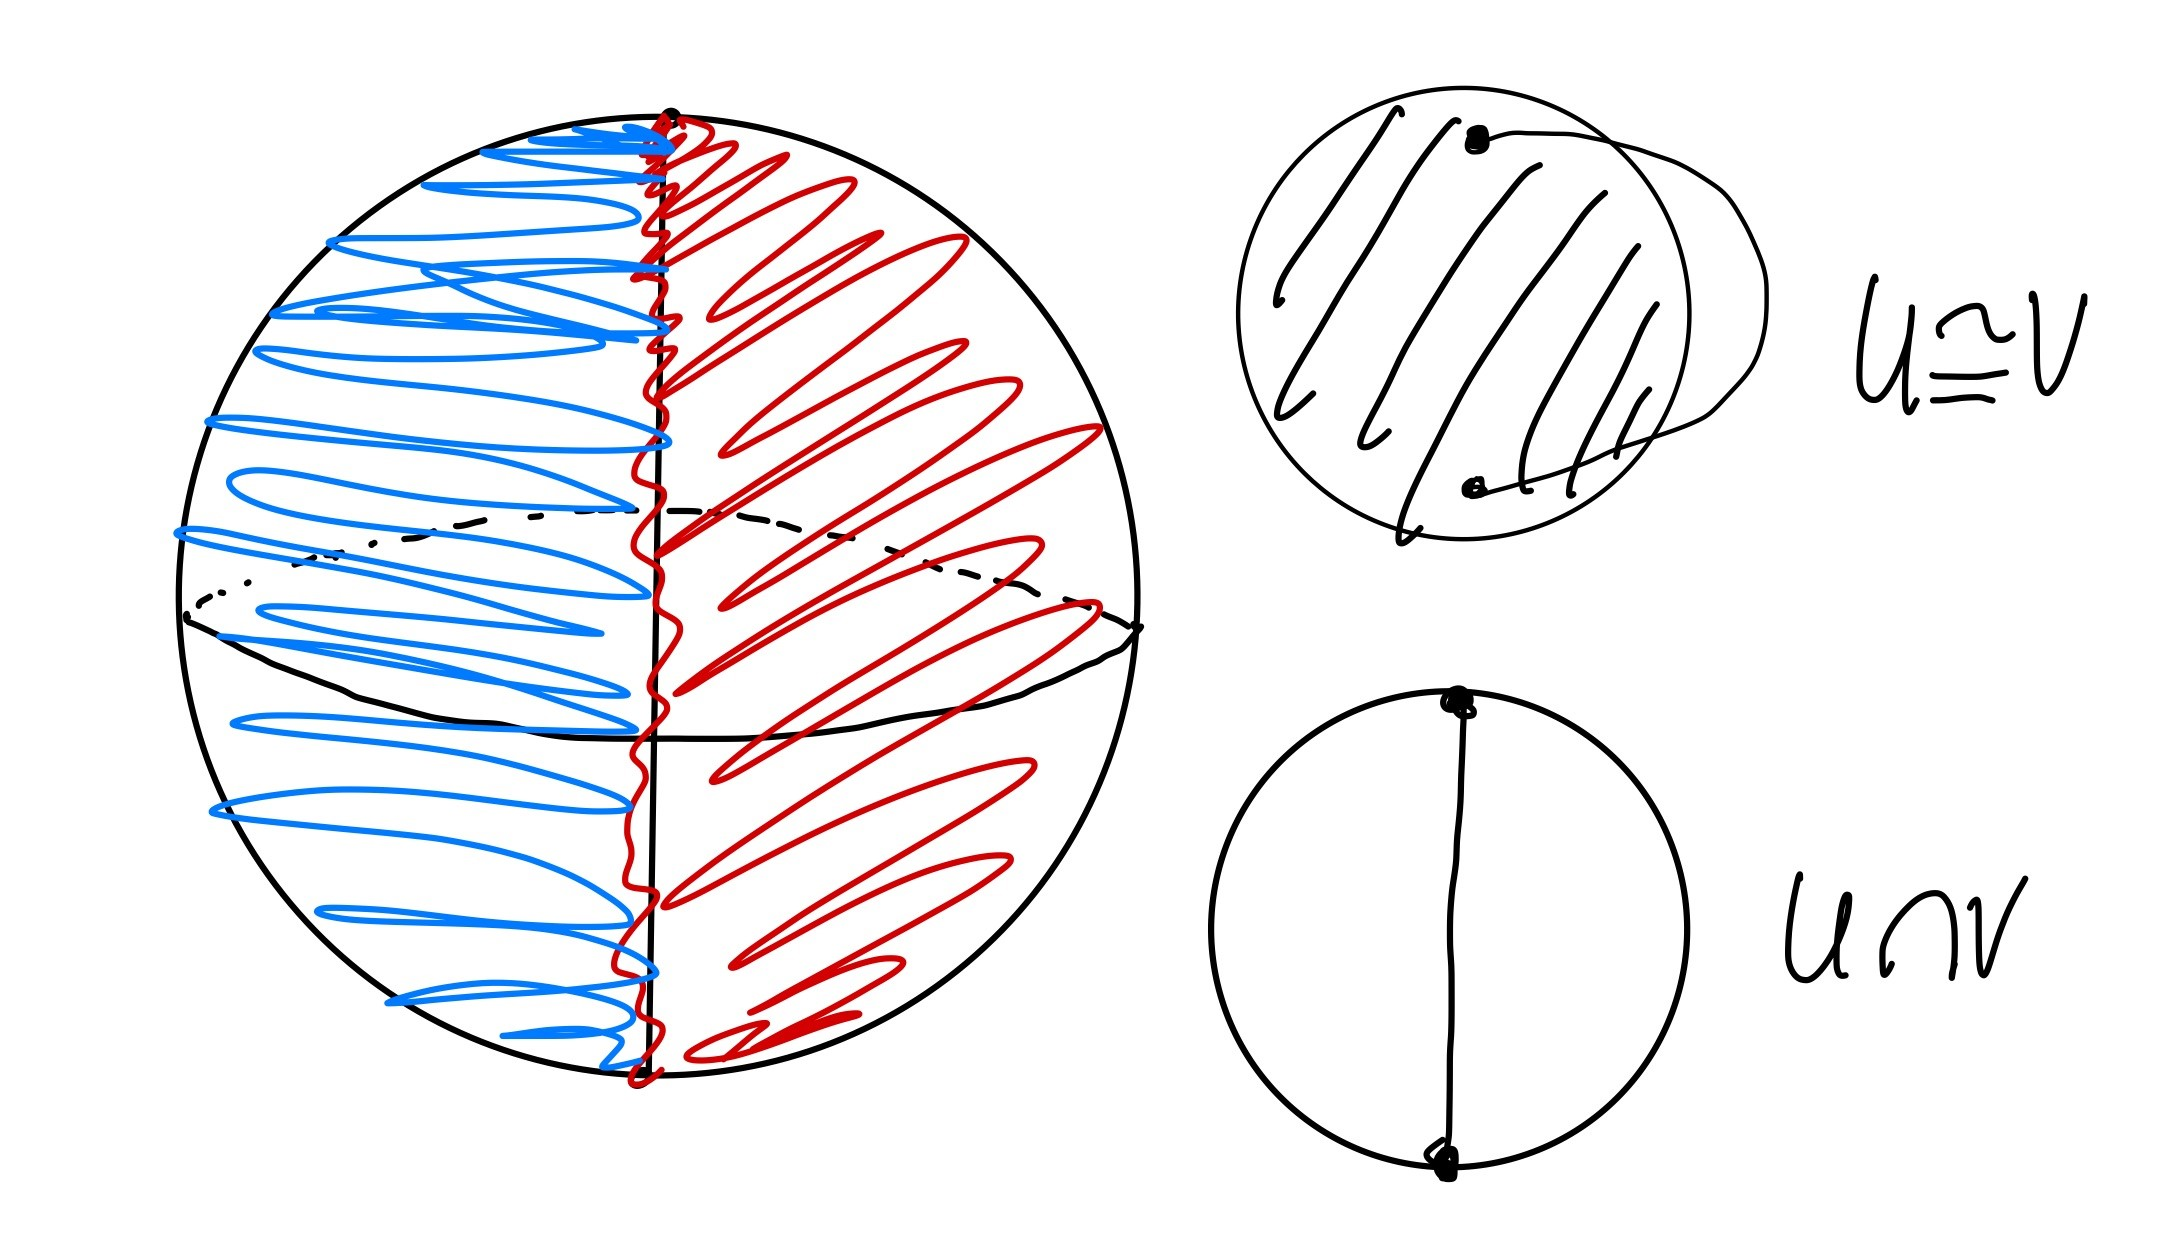
\includegraphics[scale=0.1]{Pictures/HW6-1-1.jpg}\]
We know both \(U,V,U \cap V\) are path-connected, so we assume the basepoint is chosen in \(U\cap V\) and omit the notation in the calculation. Note that \(U\cong V\simeq S^1\) and \(U\cap V\simeq S^1\vee S^1\). By Van Kampen Theorem, we have a pushout square in groups  
\[\begin{tikzcd}
	{\pi_1(S^1\vee S^1)} & {\pi_1(S^1)} \\
	{\pi_1(S^1)} & {\pi_1(X)}
	\arrow["i", from=1-1, to=1-2]
	\arrow["j"', from=1-1, to=2-1]
	\arrow[from=1-2, to=2-2]
	\arrow[from=2-1, to=2-2]
\end{tikzcd}\]
We have \(\pi_1(X)=\mathbb{Z}*\mathbb{Z}/(\im i\sim\im j)\). Note that the two maps \(i,j\) induced by inclusion \(U\cap V\hookrightarrow U\) and \(U\cap V\hookrightarrow V\). \(i\) and \(j\) have the same image by symmetry and the induced map is surjective. So \(\im i=\im j=\mathbb{Z}\). This implies 
\(\pi_1(X)=\mathbb{Z}\).
\item Let \(X\) be the quotient space of \(S^2\sqcup S^2\) where the two north poles and the two south poles are identified respectively. Same as previous. \(X\) is homotopic equivalent to the space \(S^2\sqcup S^2\) where there are two lines connecting north poles and south poles respectively. Consider \(U\) and \(V\) indicated in the pictures by red and blue. 
We can see that \(U\cong V\) is homeomorphic to two disks connected by two lines, thus homotopic equivalent to \(S^1\) since a disk is contractible. The intersection \(U\cap V\) is homotopic equivalent to two \(S^1\) connected by two lines, thus further homotopic equivalent to the wedge sum 
\(S^1\vee S^1\vee S^1\).
\[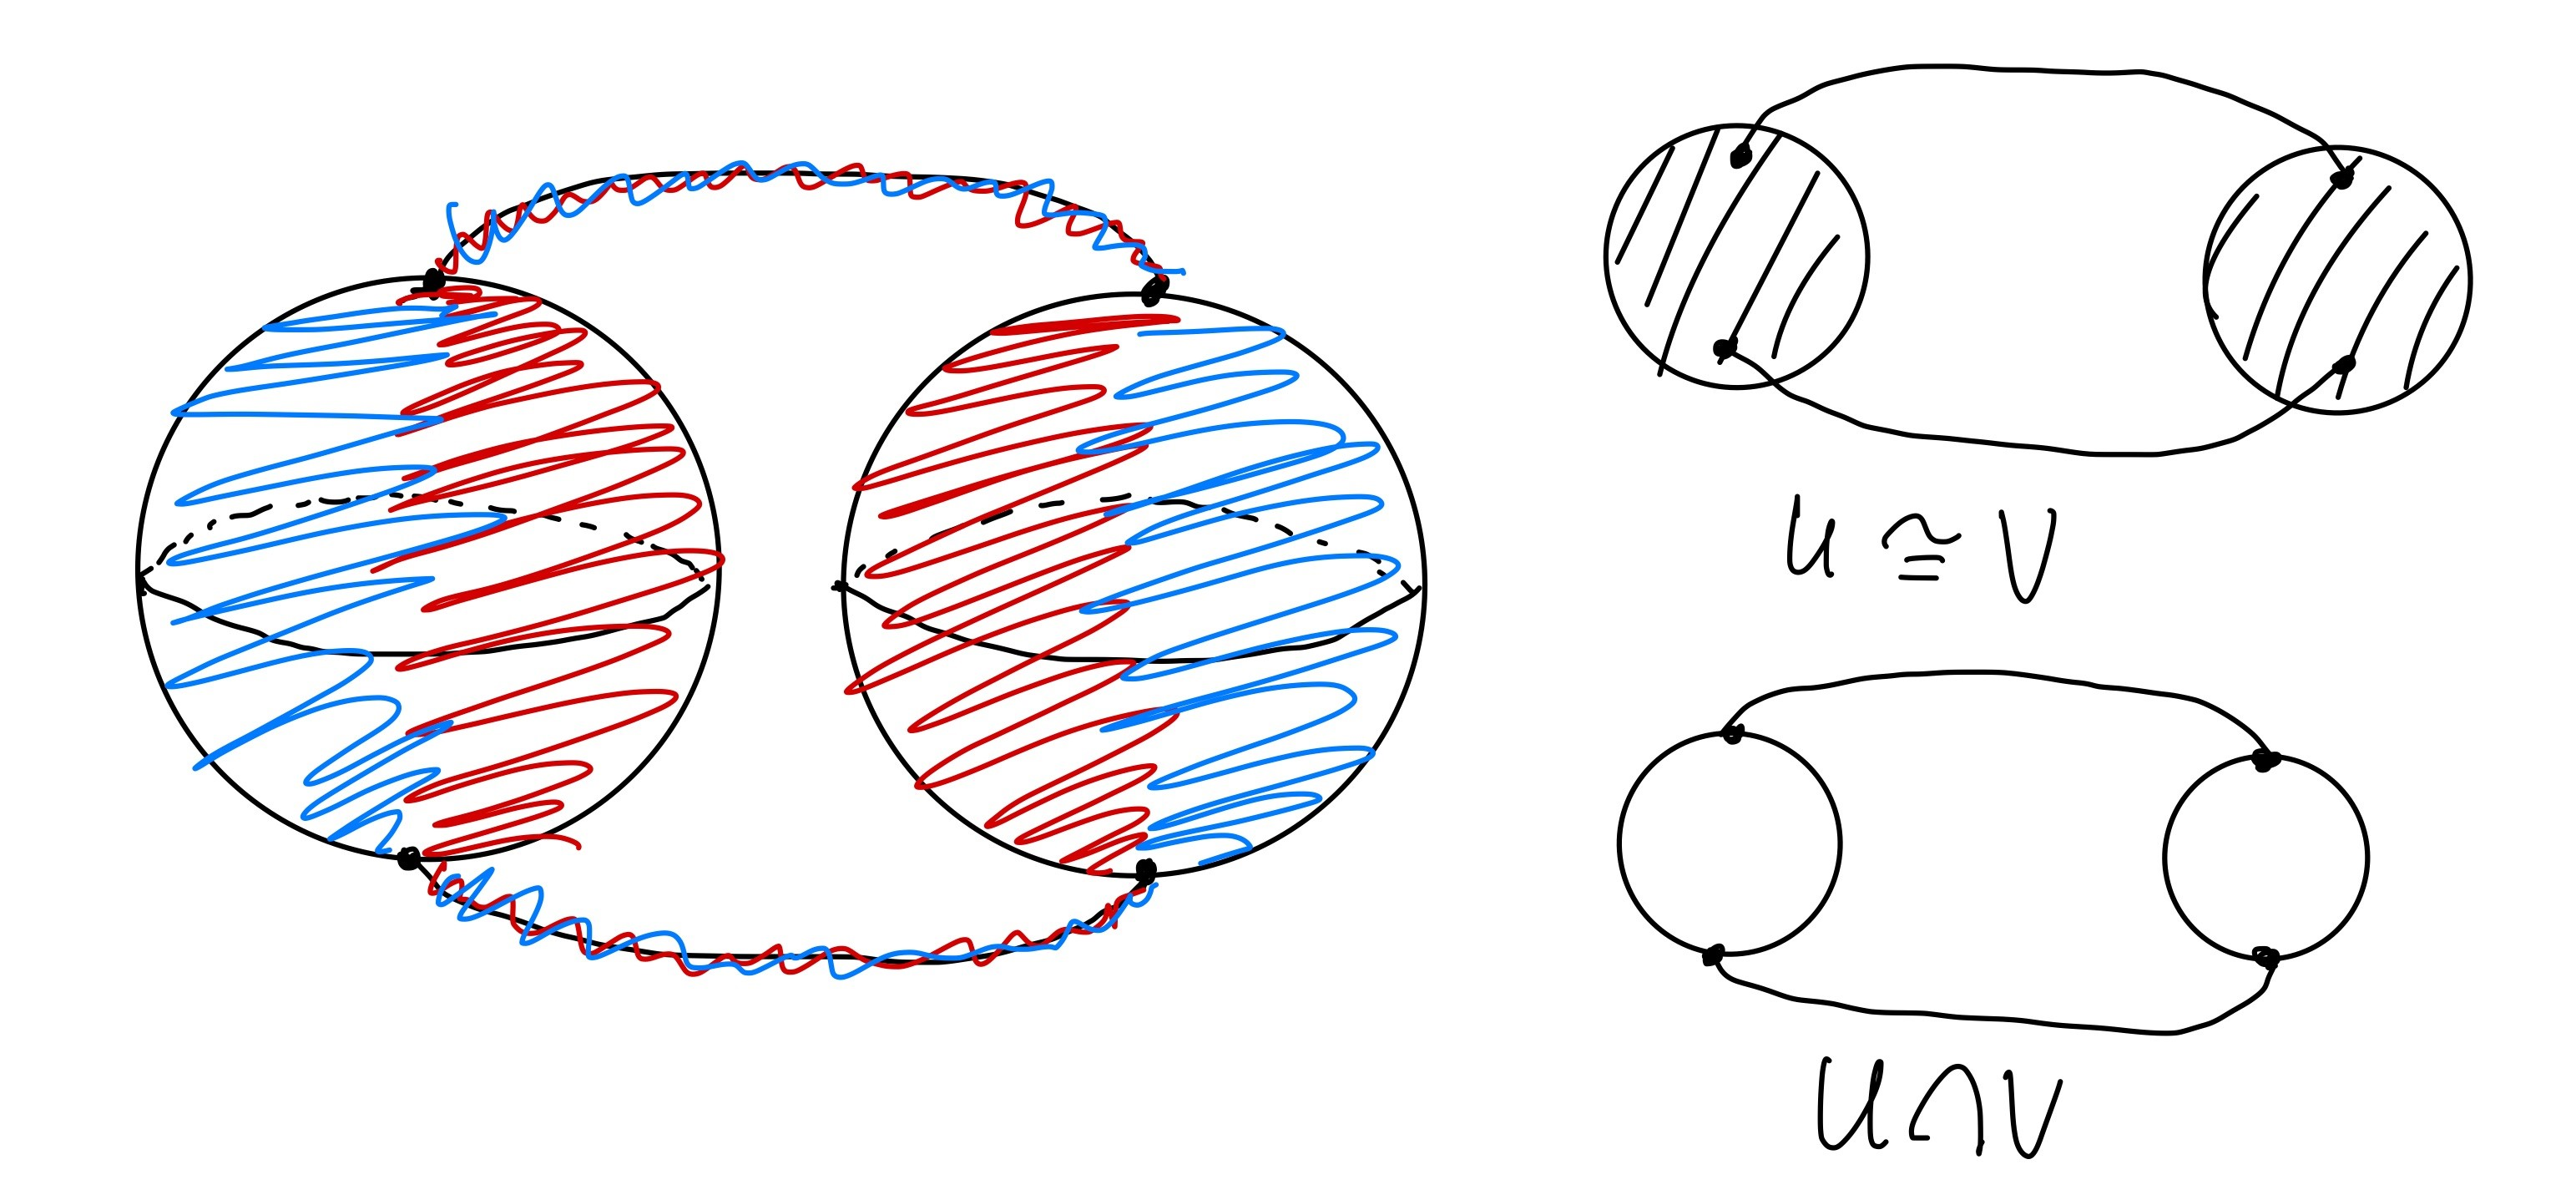
\includegraphics[scale=0.1]{Pictures/HW6-1-2.jpg}\]
We know that \(U\cap V, U, V\) are path-connected, so we assume the base point is chosen in \(V\cap U\) and omit the notation in the calculation. By Van Kampen Theorem, we have a pushout square in groups 
\[\begin{tikzcd}
	{\pi_1(S^1\vee S^1\vee S^1)} & {\pi_1(S^1)} \\
	{\pi_1(S^1)} & {\pi_1(X)}
	\arrow["i", from=1-1, to=1-2]
	\arrow["j"', from=1-1, to=2-1]
	\arrow[from=1-2, to=2-2]
	\arrow[from=2-1, to=2-2]
\end{tikzcd}\]
We have \(\pi_1(S^1\vee S^1\vee S^1)=\mathbb{Z}*\mathbb{Z}*\mathbb{Z}\). So \(\pi_1(X)=\mathbb{Z}/(\im i\sim \im j)\). \(i\) and \(j\) have the same image by symmetry and the map \(i\) must be sujective since it is induced by inclusion of spaces. So we have \(\pi_1(X)=\mathbb{Z}\). 
\item We know that \(\mathbb{R}^3\) is homotopic to \(D^3\). Let \(X\) be the space of \(D^3\) removing three lines passing through this solid ball. These three lines pass through the one common point in \(D^3\). We first remove the commom point in three lines from inside \(D^3\). Since \(D^3\) removing one point inside is homotopic equivalent to \(S^2\), we know that \(X\) is homotopic equivalent to the \(S^2\) removing 6 points. Note that 
\(S^2\cong \mathbb{R}^2\cup \left\{ \infty \right\}\). Thus, \(S^2\) removing 6 points is homotopic equivalent to \(\mathbb{R}^2\) removing 5 points. And from what we have discussed in part \((d)\), we know that \(\pi_1(X)=\underbrace{\mathbb{Z}*\cdots*\mathbb{Z}}_{5\ \text{times}}\). 
\item Let \(X\) be \(\mathbb{R}^n\) removing \(k\) points. \(X\) is always path-connected, so we omit the basepoint notation in the calculations. When \(n=2\), if \(k=0\), then \(\mathbb{R}^2\) is contractible, so \(\pi_1(\mathbb{R}^2)=*\) is trivial. If \(k\geq 1\), without loss of generality, we may assume all \(k\) points \(x_1,\ldots,x_k\) are on the circle centered at the origin with radius \(1\). We know that \(\mathbb{R}^3\) is homotopic equivalent to 
\(D^2\), which can be viewed as a disk centered at the origin with radius \(2\). Divide the disk \(D^2\) into fan-shaped sectors with having one and only one \(x_i\) inside each sector. This can be done since the points removed are discrete. Then removing each point inside the fan-shaped sector can be viewed as homotopic to removing the surfaces occupying that secton. Thus, \(X\) is 
homotopic equivalent to \(S^1\) with \(k\) lines connecting to the center. Choose the center as the basepoint and it is easy to see that \(X\) is homotopic equivalent to \(k\) copies of \(S^1\) wedged at one point. By Van Kampen Theorem and what we proved in class, we know \(\pi_1(X)=\underbrace{\mathbb{Z}*\cdots*\mathbb{Z}}_{k\  \text{times}}\). 
\[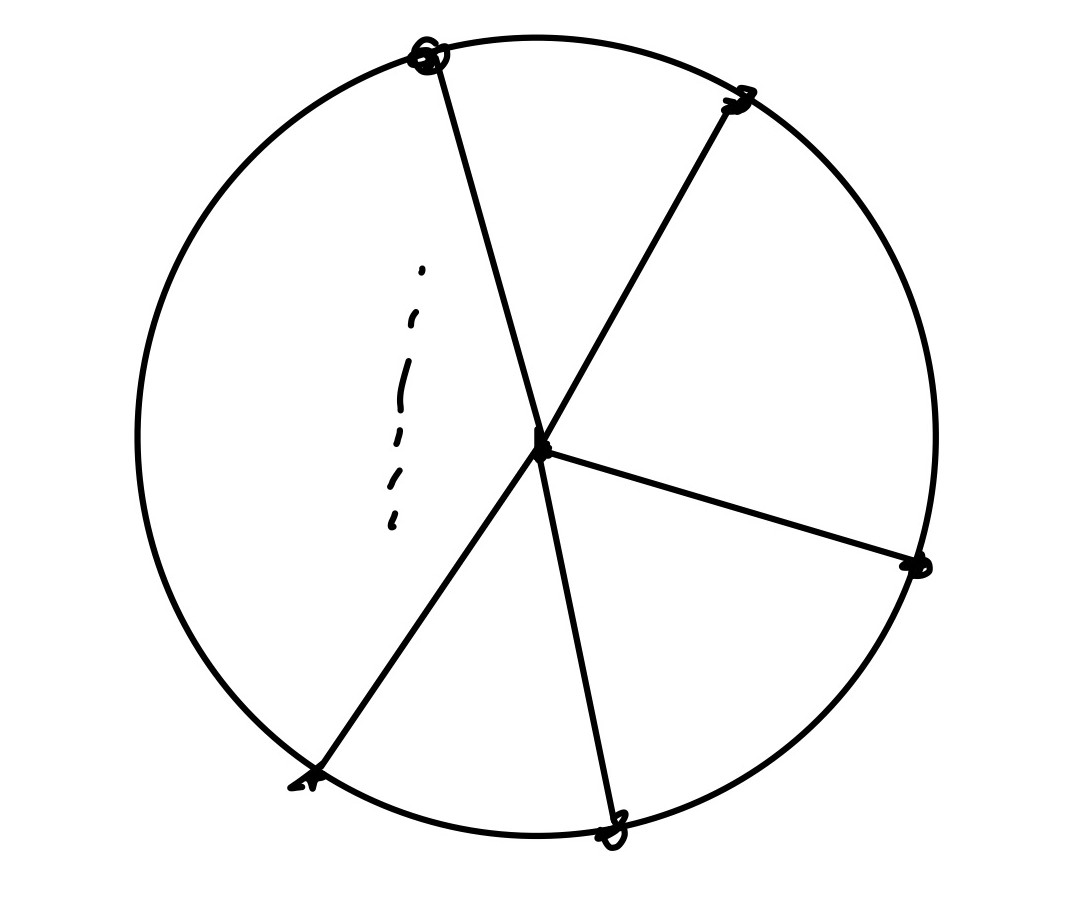
\includegraphics[scale=0.1]{Pictures/HW6-1-4.jpg}\]
Now assume \(n\geq 2\). When \(k=0\), we know that \(\mathbb{R}^n\) is contractible. So \(\pi_1(\mathbb{R}^n)=*\) is trivial. For \(k\geq 1\), using the same method as above, we can see that \(X\) is homotopic equivalent to \(k\) copies of \(S^{n-1}\) wedged at one point. For any \(n\geq 2\), \(S^{n-1}\) is simply-connected, so by Van Kampen Theorem, the wedge sum is also simply-connected. We have 
\(\pi_1(X)=*\) is trivial. To summarize, we have 
\[\pi_1(X)=\begin{cases}
    \underbrace{\mathbb{Z}*\cdots*\mathbb{Z}}_{k\ \text{times}},&\iif n=2,k\geq 1;\\
    0,&\ \ \otherwise.
\end{cases}\]
\item Let \(X\) be the space of torus \(T\) removing two points. Note that \(X\) is still path-connected, so we omit the choice of basepoint. Consider the standard cell complex structure for the torus \(T\) as shown. Additionally, the 0-cell \(x\) are connected by a red line, which is homeomorphic to \(S^1\) in the 2-cell, thus dividing the 2-cell into two sectors. Next, remove one point from each of the two sectors. \(X\) is homotopic equivalent to the \(1\)-skeleton of this cell complex, which has one \(0\)-cell \(x\), 
and three \(1\)-cells \(a,b,c\). From this we can see that \(X\) is homotopic equivalent to \(S^1\vee S^1\vee S^1\). By Van Kampen Theorem, \(\pi_1(X)=\mathbb{Z}*\mathbb{Z}*\mathbb{Z}\). 
\[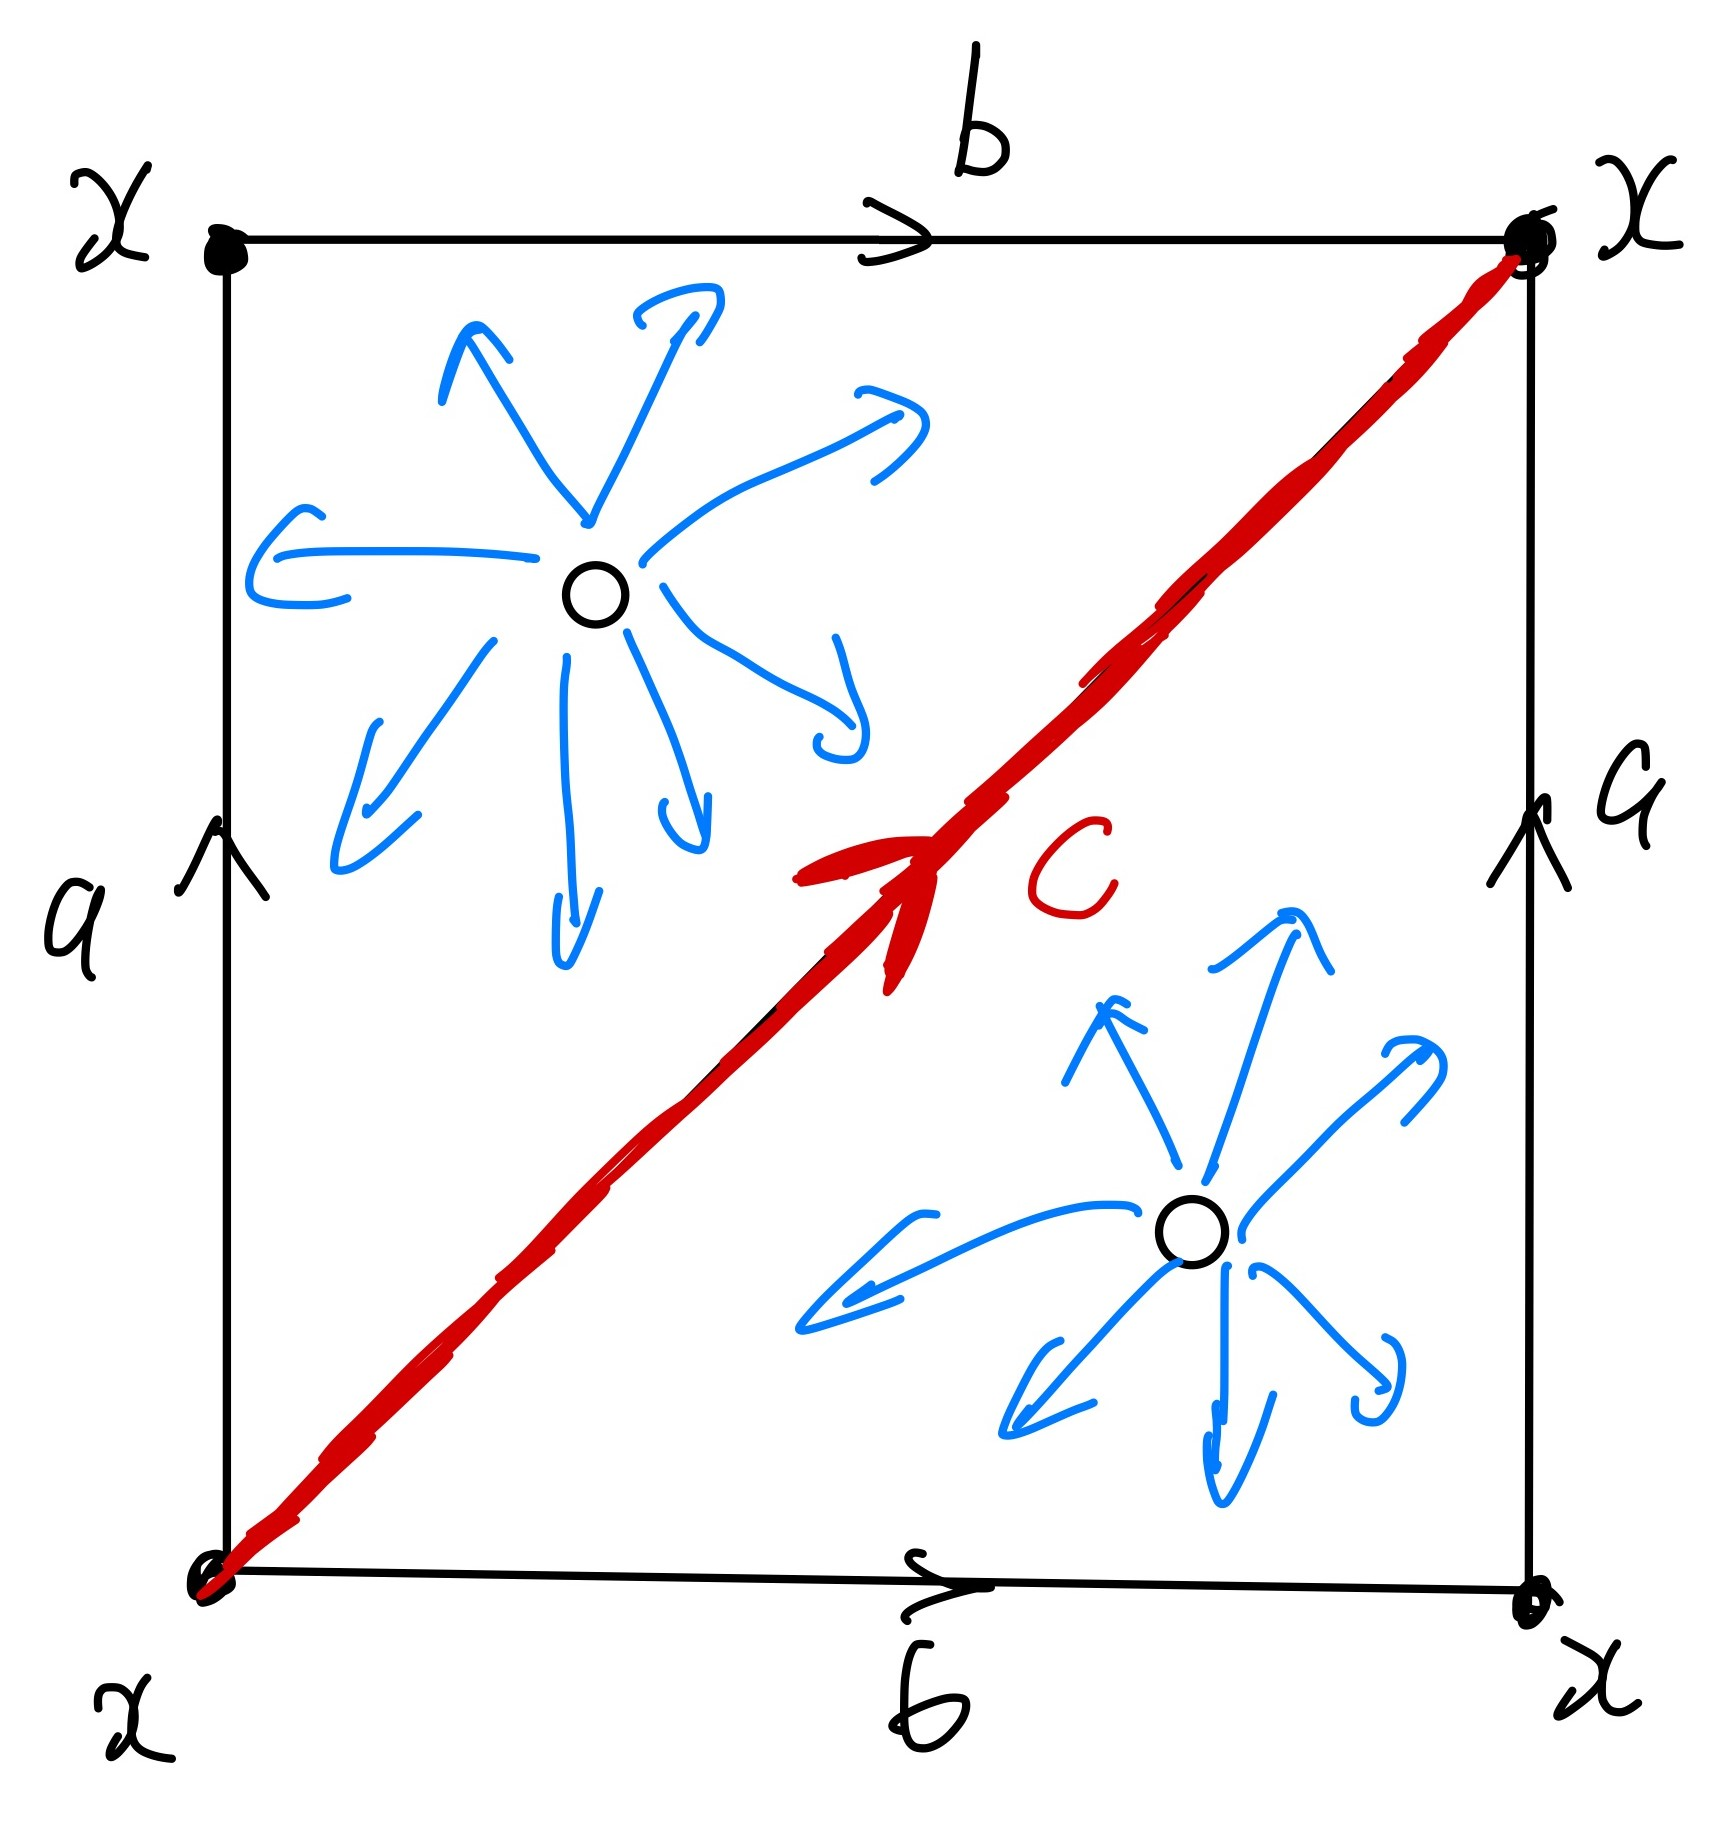
\includegraphics[scale=0.1]{Pictures/HW6-1-5.jpg}\]
\item Let \(M=S^4\times S^1\) and \(x\in M\) be a point. We know both \(S^4\) and \(S^1\) are path-connected, so \(M\) is also path-connected. We omit the choice of basepoint from now on. Note that \(M\) is a \(5\)-manifold. There exists an open neighborhood \(U\) of \(x\) in \(M\) such that 
\(U\cong \mathbb{R}^5\). Let \(V=M-\left\{ x \right\}\) which is also open in \(M\). We have 
\[U\cap V\cong U-\left\{ x \right\}\cong \mathbb{R}^5-\left\{ * \right\}.\]
So \(U\cap V\) is homotopic equivalent to \(S^4\). By Van Kampen Theorem, we have a pushout square of groups 
\[\begin{tikzcd}
	{\pi_1(S^4)} & {\pi_1(U)} \\
	{\pi_1(M-\left\{x\right\})} & {\pi_1(M)}
	\arrow[from=1-1, to=1-2]
	\arrow[from=1-1, to=2-1]
	\arrow[from=1-2, to=2-2]
	\arrow[from=2-1, to=2-2]
\end{tikzcd}\]
Note that \(\pi_1(S^4)=*\) is trivial and \(\pi_1(U)=\pi_1(\mathbb{R}^5)=* \) is also trivial. So we have 
\[\pi_1(M-\left\{ x \right\})=\pi_1(M)=\pi_1(S^4\times S^1)=\pi_1(S^4)\times \pi_1(S^1)=\mathbb{Z}.\]
\item Let \(X\) be the space of \(\mathbb{R}P^4\) removing two points. Consider the standard CW complex structure on \(\mathbb{R}P^4\). We know that \(\mathbb{R}P^4\) can be viewed as \(\mathbb{R}P^3\) attaching a \(4\)-cell \(D^4\) via a degree 0 boundary map \(S^3\rightarrow S^3\). We choose a base point \(x\in \mathbb{R}P^3\) and 
one \(S^3\) inside the interior of \(D^4\) (red in picture), denoted by \(Y\). We know that \(Y\cap \partial D^4=\left\{ x \right\}\). Choose one point inside the space bounded by \(Y\) and another point in the interior of \(D^4\) but not in \(Y\). Remove these two points and we obtain \(X\). We know that 
\(D^4\) removing these two points is homotopic equivalent to the union \(Y\cup \partial D^4\). Note that \(\partial D^4=S^3\) is glued to the 3-skeleton \(\mathbb{R}P^3\), so \(X\) is homotopic equivalent to \(\mathbb{R}P^3\vee Y=\mathbb{R}P^3\vee S^3\). 
\[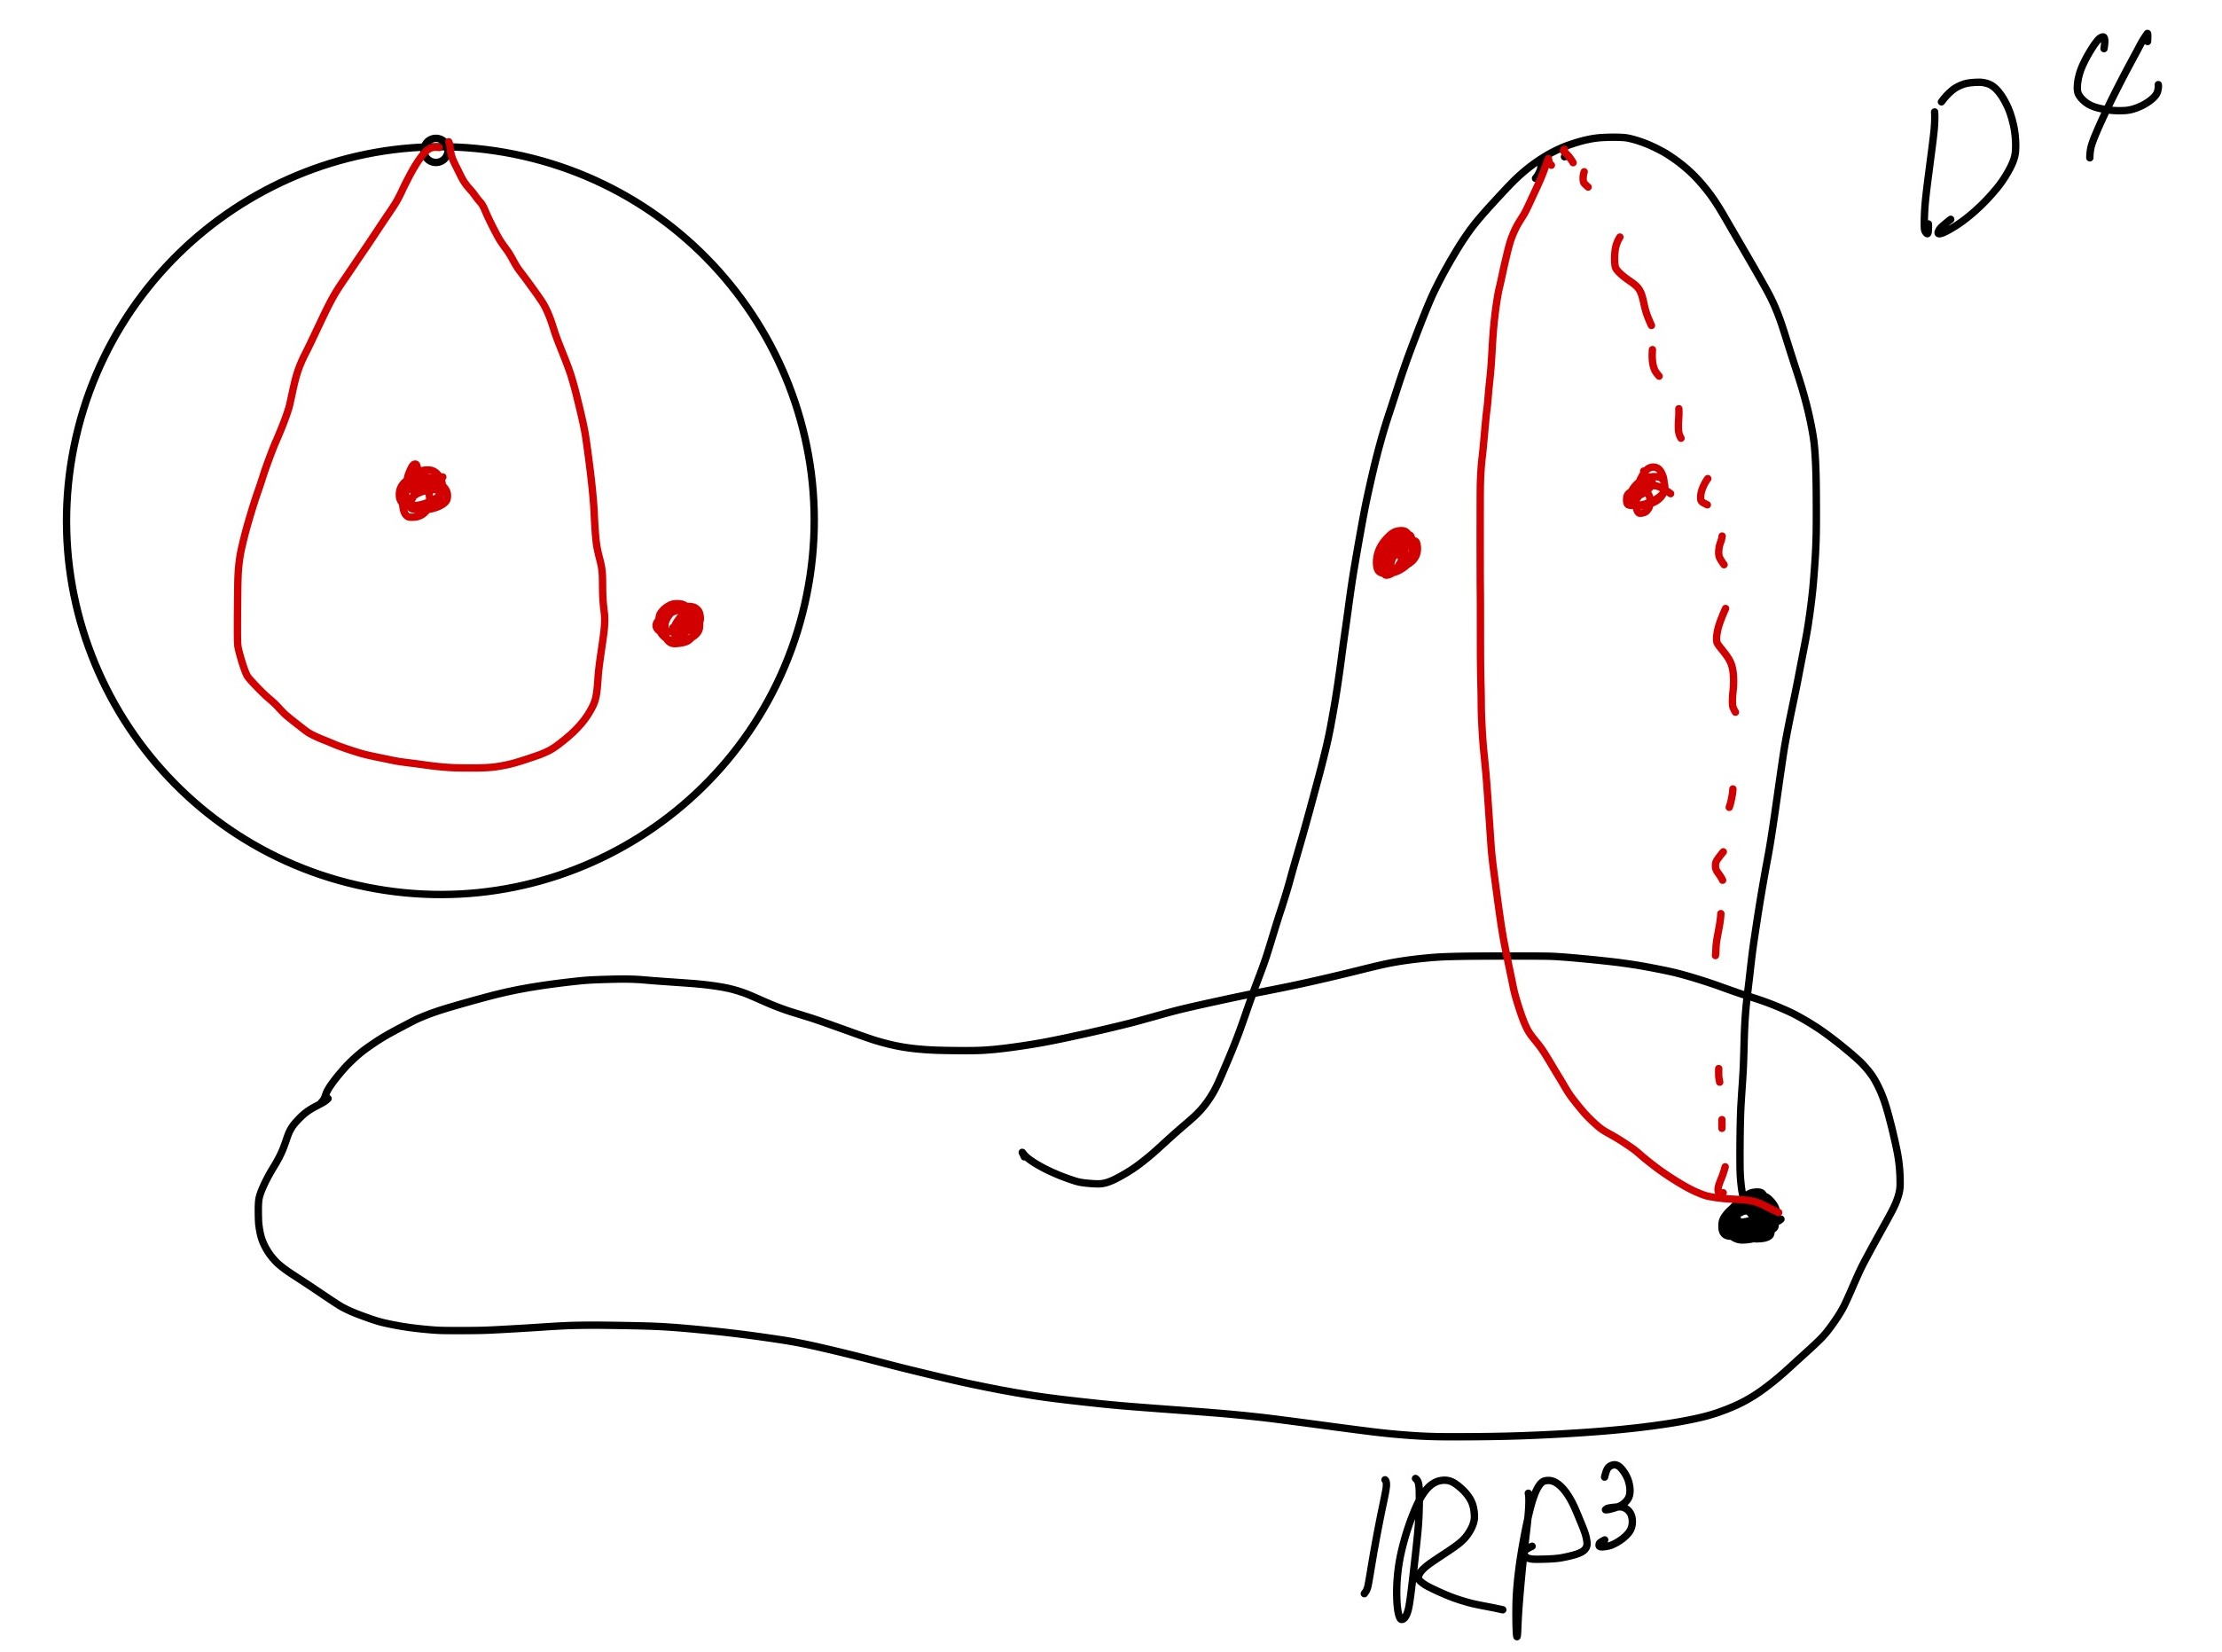
\includegraphics[scale=0.1]{Pictures/HW6-1-7.jpg}\]
By Van Kampen Theorem, we have 
\[\pi_1(X)=\pi_1(\mathbb{R}P^3)*\pi_1(\mathbb{S}^3)=\pi_1(\mathbb{R}P^3).\]
We know \(\mathbb{R}P^2\) is the 2-skeleton of \(\mathbb{R}P^3\), so \(\pi_1(X)=\pi_1(\mathbb{R}P^3)\cong \pi_1(\mathbb{R}P^2)=\mathbb{Z}/2 \mathbb{Z}\).
\end{enumerate} 
\end{solution}

\noindent\rule{7in}{2.8pt}
%%%%%%%%%%%%%%%%%%%%%%%%%%%%%%%%%%%%%%%%%%%%%%%%%%%%%%%%%%%%%%%%%%%%%%%%%%%%%%%%%%%%%%%%%%%%%%%%%%%%%%%%%%%%%%%%%%%%%%%%%%%%%%%%%%%%%%%%
%Probelm 2
%%%%%%%%%%%%%%%%%%%%%%%%%%%%%%%%%%%%%%%%%%%%%%%%%%%%%%%%%%%%%%%%%%%%%%%%%%%%%%%%%%%%%%%%%%%%%%%%%%%%%%%%%%%%%%%%%%%%%%%%%%%%%%%%%%%%%%%%
\begin{problem}{2}
Let \(p\) and \(q\) be relatively prime, positive integers. Consider the \(3\)-disk \(D^3\subseteq \mathbb{R}^3\), and regard it as the space 
\[D^3=\left\{ (z,r)\mid z\in \mathbb{C}, r\in \mathbb{R}, |z|^2+r^2\leq 1\right\}.\]
Let  \(\zeta=e^{2\pi i/p}\), and let \(L(p,q)\) be the quotient space of \(X\) where one identifies 
\[(z,r)\sim (\zeta^qz,-r)\]
if \(r\geq 0\) and \(|z|^2+r^2=1\). Convince yourself that \(L(p,q)\) is a 3-manifold. The space \(L(p,q)\) is called a lens space. Note that \(L(2,1)=\mathbb{R}P^3\). \\ 
Let \(\rho:D^3\rightarrow L(p,q)\) be the quotient map. Let 
\begin{align*}
    X_0=&\left\{ \rho(1,0) \right\},\\ 
    X_1=&\left\{ \rho(z,0)\mid z\in \mathbb{C},|z|^2=1 \right\},\\ 
    X_2=&\left\{ \rho(z,r)\mid |z|^2+r^2=1 \right\}.
\end{align*}
Convince yourself that 
\[\varnothing \hookrightarrow X_0\hookrightarrow X_1\hookrightarrow X_2\hookrightarrow X_3=L(p,q)\]
 is a CW-structure on \(L(p,q)\), with exactly one cell in each dimension. Use this to compute \(H_*(L(p,q))\) as well as \(\pi_1(L(p,q))\).
\end{problem}
\begin{solution}
The solutions are divided into three parts. In part (1), we prove that \(L(p.q)\) is indeed a \(3\)-manifold. In part (2), we prove that the given structure in the problem is a CW structure on \(L(p,q)\). Lastly, 
in part (3), we calculate the homology and fundamental groups of \(L(p,q)\).
\begin{enumerate}[(1)]
\item We have already know that \(D^3\) is a \(3\)-manifold with boundary, to show that \(L(p,q)\) is a \(3\)-manifold, we need to show that for every point \((z,r)\in \partial D^3\) with \(|z|=1\), after the identification, it has 
an open neighborhood which is homeomorphic to \(\mathbb{R}^3\). For points \((z,r)\) satisfying \(r< 0\), it is identifies with exactly one point in the upper half sphere, so it has  a neighborhood homeomorphic to \(\mathbb{R}^3\). For each 
point \((z,0)\) with \(|z|^2=1\) on the equator, note that if we choose an open neighborhood small enough, no points in this neighborhood are identified with each other, so we can piece together \(p-1\) such neighborhood to get \(\mathbb{R}^3\) as 
each of them can be chosen as being homeomorphic to a half ball.
\item It is easy to see that \(X_0\) is just a point and \(X_1\) just \(S^1\) with \(|z|=1\) and \(r=0\) in \(L(p,q)\). Note that for point \(z\in L(p,q)\) satisfying \(|z|=1\), we identify the points \(z\) with \(e^{2\pi i\frac{q}{p}}z\). Since \(p\) and \(q\) are 
coprime, we divide this circle into \(p\) copies of \(S^1\) and view them as just one \(S^1\). When attaching a \(2\)-cell to \(X_1\), we use a degree \(p\) map \(S^1\rightarrow S^1\). Note that we only have one \(2\)-cell because if \(L(p,q)\) is viewed as a quotient space \(D^3/\sim\), 
for \(r\geq 0\), all points \((z,r)\) in lower half sphere in \(\partial D^3\) is identified with a point \((e^{2\pi i \frac{q}{p}}z,-r)\) in the upper half sphere. Finally, we attach a \(3\)-cell to the \(2\)-skeleton \(X_2\), which corresponding to the interior of the quotient space \(D^3/\sim\). This gives us 
a CW structure for \(L(p,q)\):
\[\varnothing \hookrightarrow X_0\hookrightarrow X_1\hookrightarrow X_2\hookrightarrow X_3=L(p,q).\]
\item The cellular chain complex from the above CW structure is given by 
\[0\rightarrow \mathbb{Z}\xrightarrow{d_3}\mathbb{Z}\xrightarrow{p}\mathbb{Z}\xrightarrow{0}\mathbb{Z}\rightarrow 0.\]
Note that \(d_3=0\) because this is a chain complex. So the homology can be calculated as 
\[H_i(L(p,q))=\begin{cases}
    \mathbb{Z},&\iif i=0,3;\\ 
    \mathbb{Z}/ p \mathbb{Z},&\iif i=1;\\
    0,&\ \otherwise.
\end{cases}\]
For the fundamental group \(\pi_1(L(p,q))\), from the CW structure, we know that \(\pi_1(L(p,q))=\pi_1(X_2)=\pi_1(X_1)/\sim\) where \(\sim\) is given by the attaching map \(S^1\rightarrow S^1\). We have seen that it is a degree \(p\) map, so the fundamental group 
\(\pi_1(L(p,q))=\mathbb{Z}/p \mathbb{Z}\).
\end{enumerate}
\end{solution}

\noindent\rule{7in}{2.8pt}
%%%%%%%%%%%%%%%%%%%%%%%%%%%%%%%%%%%%%%%%%%%%%%%%%%%%%%%%%%%%%%%%%%%%%%%%%%%%%%%%%%%%%%%%%%%%%%%%%%%%%%%%%%%%%%%%%%%%%%%%%%%%%%%%%%%%%%%%
%Probelm 3
%%%%%%%%%%%%%%%%%%%%%%%%%%%%%%%%%%%%%%%%%%%%%%%%%%%%%%%%%%%%%%%%%%%%%%%%%%%%%%%%%%%%%%%%%%%%%%%%%%%%%%%%%%%%%%%%%%%%%%%%%%%%%%%%%%%%%%%%
\begin{problem}{3}
Suppose \(W\) is a space and \(h:W\rightarrow W\) is a homeomorphism. Let \(X\) be the quotient space of \(W\times I\) where we identify \((w,0)\sim (h(w),1)\) for all \(w\in W\). Note that 
if \(W\) is a \(d\)-manifold then \(X\) is a \((d+1)\)-manifold. If \(W=S^2\) then \(\deg(h)\) is either \(1\) or \(-1\). Compute \(H_*(X)\) in both cases. 
\end{problem}
\begin{solution}
Let \(X\) be the quotient space of \(S^2\times I\) obtained in this way. Consider the open sets \(U=S^2\times (\frac{1}{4},\frac{3}{4})\) and \(V=S^2\times ((0,\frac{1}{3})\cup (\frac{2}{3},1))\). We have \(X=U\cup V\). Note that \(S^2\times \left\{ 0 \right\}\) is identified with 
\(S^2\times \left\{ 1 \right\}\) via a homeomorphism \(h\), so we know that both \(U\) and \(V\) are homotopic equivalent to \(S^2\). Moreover, we have 
\[U\cap V=S^2\times ((\frac{1}{4},\frac{1}{3})\cup(\frac{2}{3},\frac{3}{4}))\simeq S^2\sqcup S^2.\]
By Mayer-Vietoris, we have a long exact sequence in homology 
\[\begin{tikzcd}
	& {\tilde{H}_*(U\cap V)} & {\tilde{H}_*(U)\oplus \tilde{H}_*(V)} & {\tilde{H}_*(X)} \\
	3 & 0 & 0 & {?} \\
	2 & {\mathbb{Z}\oplus\mathbb{Z}} & {\mathbb{Z}\oplus\mathbb{Z}} & {?} \\
	1 & 0 & 0 & {?} \\
	0 & {\mathbb{Z}} & 0
	\arrow[from=2-2, to=2-3]
	\arrow[from=2-3, to=2-4]
	\arrow[from=2-4, to=3-2]
	\arrow["{i_*,j_*}"', from=3-2, to=3-3]
	\arrow[from=3-3, to=3-4]
	\arrow[from=3-4, to=4-2]
	\arrow[from=4-2, to=4-3]
	\arrow[from=4-3, to=4-4]
	\arrow[from=4-4, to=5-2]
	\arrow[from=5-2, to=5-3]
\end{tikzcd}\]
It can be observed that 
\[H_1(X)\cong \tilde{H}_0(U\cap V)=\tilde{H}_0(S^2\sqcup S^2)=\mathbb{Z}.\]
\(X\) is path-connected since \(S^2\times I\) is path-connected, so \(H_0(X)=\mathbb{Z}\). For the rest of the homology groups, we need to determine the map in homology 
\[H_2(S^2\sqcup S^2)\rightarrow H_2(S^2)\oplus H_2(S^2)\]
which is induced by the inclusion \(i:U\cap V\rightarrow U\) and \(j:U\cap V\rightarrow V\). Choose the spheres \(S^2\times \left\{ \frac{2}{7} \right\}\) and 
\(S^2\times \left\{ \frac{5}{7} \right\}\) in \(U\cap V\) as the generators of the homology group \(H_2(U\cap V)=\mathbb{Z}\oplus \mathbb{Z}\). We know that \(H_2(U)=H_2(S^2)=\mathbb{Z}\) has only one generator, so the spheres at \(S^2\times \left\{  \frac{2}{7}\right\}\) and the sphere 
at \(S^2\times \left\{ \frac{5}{7} \right\}\) is the same generator in \(H_2(U)\), so \(i_*\) can be described as 
\begin{align*}
    i_*:\mathbb{Z}\oplus \mathbb{Z}&\rightarrow \mathbb{Z};\\ 
        (1,0)&\mapsto 1,\\ 
        (0,1)&\mapsto 1.
\end{align*}
For \(V\), we know \(H_2(V)=\mathbb{Z}\) have one generator and we choose the sphere at \(S^2\times \left\{ \frac{5}{7} \right\}\). So one of the generator \(S^2\times \left\{ \frac{5}{7} \right\}\) of \(H_*(U\cap V)\) is sent to itself, and for the other generator \(S^2\times \left\{ \frac{2}{7} \right\}\), firstly it is sent to the sphere at 
\(S^2\times \left\{ 0 \right\}\), then the induced map in homology \(h_*:H_2(S^2)\rightarrow H_2(S^2)\) sends it to the homology group of the sphere at \(S^2\times \left\{ 1 \right\}\), which is the same as the generator at \(S^2\times \left\{ \frac{5}{7} \right\}\). Note that 
\(\deg h\) is just how we sent \(1\in H_2(S^2)\), so \(j_*\) can be described as 
\begin{align*}
    j_*:\mathbb{Z}\oplus \mathbb{Z}&\rightarrow \mathbb{Z};\\ 
    (1,0)&\mapsto \deg h,\\ 
    (0,1)&\mapsto 1.
\end{align*}
So the map in homology \(H_2(S^2\sqcup S^2)\xrightarrow{i_*,j_*}H_2(S^2)\oplus H_2(S^2)\) can be summarized as a matrix \(\begin{pmatrix}
    1&\deg h\\ 
    1&1
\end{pmatrix}\). Note that \(H_3(X)=\ker (i_*,j_*)\) and \(H_2(X)=\coker (i_*,j_*)\).\\ 
When \(\deg h=1\), the matrix is similar to \(\begin{pmatrix}
    1&0\\ 
    0&0
\end{pmatrix}\) and we have 
\[H_i(X)=\begin{cases}
    \mathbb{Z},&\iif i=0,1,2,3;\\ 
    0,&\ \otherwise.
\end{cases}\]
And when \(\deg h=-1\), the matrix is similar to \(\begin{pmatrix}
    1&0\\ 
    0&2
\end{pmatrix}\) and we have 
\[H_i(X)=\begin{cases}
    \mathbb{Z},&\iif i=0,1;\\ 
    \mathbb{Z}/2 \mathbb{Z},&\iif i=2;\\
    0,&\ \otherwise.
\end{cases}\]
\end{solution}

\noindent\rule{7in}{2.8pt}
%%%%%%%%%%%%%%%%%%%%%%%%%%%%%%%%%%%%%%%%%%%%%%%%%%%%%%%%%%%%%%%%%%%%%%%%%%%%%%%%%%%%%%%%%%%%%%%%%%%%%%%%%%%%%%%%%%%%%%%%%%%%%%%%%%%%%%%%
%Probelm 4
%%%%%%%%%%%%%%%%%%%%%%%%%%%%%%%%%%%%%%%%%%%%%%%%%%%%%%%%%%%%%%%%%%%%%%%%%%%%%%%%%%%%%%%%%%%%%%%%%%%%%%%%%%%%%%%%%%%%%%%%%%%%%%%%%%%%%%%%
\begin{problem}{4}
Regard \(\mathbb{R}^7\) as contained in \(\mathbb{R}^8\) in the usual way. For every line \(\ell\) through the origin in \(\mathbb{R}^8\), I want to associate a line \(F(\ell)\) through the origin in \(\mathbb{R}^7\). 
I want this assignment to be continous, and when \(\ell\subseteq \mathbb{R}^7\), I want \(F(\ell)=\ell\). Prove that no such assignment \(F\) can exist.
\end{problem}
\begin{solution}
Recall that for \(n\geq 2\), each point in \(\mathbb{R}P^n\) can be viewed as a line through the origin in \(\mathbb{R}^{n+1}\). To get the map \(F\) described in the problem, it is the same as defining a continous map \(f:\mathbb{R}P^7\rightarrow \mathbb{R}P^6\). \(F\) restricted to 
lines in \(\mathbb{R}^7\) being the identity means that \(f\) restricted to \(\mathbb{R}P^6\) is the identity map. Namely we have a commutative diagram 
\[\begin{tikzcd}
	{\mathbb{R}P^7} & {\mathbb{R}P^6} \\
	{\mathbb{R}P^6}
	\arrow["f", from=1-1, to=1-2]
	\arrow["i", tail, from=2-1, to=1-1]
	\arrow["id"', from=2-1, to=1-2]
\end{tikzcd}\]
where \(i:\mathbb{R}P^6\rightarrow \mathbb{R}P^7\) is the inclusion map. Apply \(\pi_6(-,*)\), and we have a commutative diagram in homotopy groups 
\[\begin{tikzcd}
	{\pi_6(\mathbb{R}P^7,*)} & {\pi_6(\mathbb{R}P^6,*)} \\
	{\pi_6(\mathbb{R}P^6,*)}
	\arrow["{f_*}", from=1-1, to=1-2]
	\arrow["{i_*}", tail, from=2-1, to=1-1]
	\arrow["id"', from=2-1, to=1-2]
\end{tikzcd}\]
Note that for \(\pi_6(\mathbb{R}P^6)=\pi_6(S^6)=\mathbb{Z}\) and \(\pi_6(\mathbb{R}P^7)=\pi_6(S^7)=0\). So this diagram cannot commute since the identity map cannot be obtained from the zero map 
composed with anything.
\end{solution}

\noindent\rule{7in}{2.8pt}
%%%%%%%%%%%%%%%%%%%%%%%%%%%%%%%%%%%%%%%%%%%%%%%%%%%%%%%%%%%%%%%%%%%%%%%%%%%%%%%%%%%%%%%%%%%%%%%%%%%%%%%%%%%%%%%%%%%%%%%%%%%%%%%%%%%%%%%%
%Probelm 5
%%%%%%%%%%%%%%%%%%%%%%%%%%%%%%%%%%%%%%%%%%%%%%%%%%%%%%%%%%%%%%%%%%%%%%%%%%%%%%%%%%%%%%%%%%%%%%%%%%%%%%%%%%%%%%%%%%%%%%%%%%%%%%%%%%%%%%%%
\begin{problem}{5}
Let \(V\) be a finite dimensional real vector space and assume it's equipped with a continous product \(V\times V\rightarrow V\) satisfying the following three conditions:
\begin{enumerate}[(i)]
\item \((rv)\cdot w=r(v\cdot w)=v\cdot (rw)\) for all \(v,w\in V\), \(r\in \mathbb{R}\); 
\item There exists an element \(1\in V\) such that \(1\cdot v=v\cdot 1=v\) for all \(v\in V\); 
\item \(vw=0\) if and only if either \(v=0\) or \(w=0\).
\end{enumerate}
Pick a basis \(e_1,\ldots,e_n\) for \(V\) such that \(e_1=1\), and define a norm on \(V\) by \
\[||r_1e_1+\cdots+r_ne_n||=\sqrt{r_1^2+\cdots+r_n^2}.\]
Let \(S(V)=\left\{ v\in V:||v||=1 \right\}\).
\begin{enumerate}[(a)]
\item Show that under our assumptions on \(V\) there is a continous map \(\theta:S(V)\times S(V)\rightarrow S(V)\) with the property that \(\theta(-1,v)=-v\) and \(\theta(1,v)=v\) for all \(v\in S(V)\). 
\item Use part (a) to show that if \(\dim_{\mathbb{R}}V\geq 2\), then the identity map \(S(V)\rightarrow S(V)\) is homotopic to the antipodal map. Conclude that \(\dim_{\mathbb{R}}V\) is either even or equal to \(1\).
\end{enumerate}
\end{problem}
\begin{solution}
\begin{enumerate}[(a)]
\item For any \(v,w\in S(V)\), we define \(\theta(v,w)=\dfrac{v\cdot w}{||v\cdot w||}\). This map is a well-defined map from \(S(V)\times S(V)\) to \(S(V)\) because 
\[||\theta(v,w)||=\dfrac{||v\cdot w||}{||v\cdot w||}=1.\]
For any \(v\in S(V)\), suppose \(v=r_1e_1+\cdots+r_ne_n\) satisfying \(r_1^2+\cdots+r_n^2=1\). We have 
\[(-1)\cdot v=-(1\cdot v)=-v=-r_1e_1-r_2e_2-\cdots-r_ne_n.\]
So we know that 
\[||-v||=\sqrt{(-r_1)^2+\cdots+(-r_n)^2}=\sqrt{r_1^2+\cdots+r_n^2}=1.\]
We can calculate 
\begin{align*}
    \theta(1,v)&=\dfrac{1\cdot v}{||1\cdot v||}=\dfrac{v}{||v||}=v,\\ 
    \theta(-1,v)&=\dfrac{(-1)\cdot v}{||(-1)\cdot v||}=\dfrac{-v}{||-v||}=-v.
\end{align*}
The last thing we need to show is that \(\theta\) define in this way is continous for all \((v,w)\in S(V)\times S(V)\). Since \(\theta\) is symmetric, we only need to show that for any \(w\in S(V)\), 
\(\theta(-,w):S(V)\rightarrow S(V)\) is a continous function. 
\item Suppose \(\dim_{\mathbb{R}}V\geq 2\). For any \(-1\leq t\leq 1\), define \(w(t)=te_1+\sqrt{1-t^2}e_2\in S(V)\), which can be viewed as a continous function of \(t\). We have a map 
\begin{align*}
    H:S(V)\times [-1,1]&\rightarrow S(V),\\ 
    (v,t)&\mapsto \theta(v,w(t)). 
\end{align*}
This map is continous because \(w\) and \(\theta\) are continous. For any \(v\in S(V)\), we can see that  
\[H(v,-1)=\theta(v,w(-1))=\dfrac{(-1)\cdot v}{||(-1)\cdot v||}=-v\]
is the antipodal map and 
\[H(v,1)=\theta(v,w(1))=\dfrac{1\cdot v}{||1\cdot v||}=v\]
is the identity map. This proves that if \(\dim_{\mathbb{R}}V\geq 2\), the identity map \(S(V)\rightarrow S(V)\) is homotopic to the antipodal map. Suppose \(\dim_{\mathbb{R}}V=n\geq 2\). We know that \(S(V)\cong S^{n-1}\). So 
the degree of the identity map \(S(V)\xrightarrow{id}S(V)\) is \(1\) and the degree of the antipodal map is \((-1)^{n-1+1}=(-1)^n\). Thus, this implies \(n\) must be even if \(n\geq 2\). We know that we have a product for \(1\)-dimensional 
real vector space because in this case, \(V\) is isomorphic to \(\mathbb{R}\), and \(\mathbb{R}\) is a field. 
\end{enumerate}
\end{solution}

\end{document}
